%%%%%%%%%%%%%%%%%%%%%%%%%%%%%%%%%%%%%%%%%%%%%%%%%%%%%%%%%%%%%%%%%%%%%%
\begin{frame}[fragile]\frametitle{}
\begin{center}
{\Large Dynamic Programming}
\end{center}

\end{frame}


%%%%%%%%%%%%%%%%%%%%%%%%%%%%%%%%%%%%%%%%%%%%%%%%%%%%%%%%%%%%%%%%%%%%%%
\begin{frame}
	\frametitle{Introduction}
		
			\begin{itemize}
			\item Dynamic programming is nothing but recursion + memoization
				\item Extension of recursion that further optimists time complexity by storing intermediate values of 
recursion so they don’t have to be re-computed. 
				\item The array/structure that stores these values is 
called a memo, and the process of storing them memoization. 
				\item A ``bottom up” approach uses 
``tabulation” instead of ``memoisation''. 
				\item Memoization is ``top-down'' because, like in the fib(n) 
example, you compute $fib(5)$ before looking for $fib(4)$ which is needed to compute $fib(5)$, whereas a 
bottom-up approach finds $fib(4)$ and puts it in a variable/array before using it to computer $fib(5)$ at 
all. 
				\item Tabulation is more efficient when all sub-problems must be solved at least once to get the final 
result (as in the $fib(n)$ problem) but memoization is faster otherwise because it strictly only 
computers things that need to be computed. 
			\end{itemize}
\end{frame}

%%%%%%%%%%%%%%%%%%%%%%%%%%%%%%%%%%%%%%%%%%%%%%%%%%%%%%%%%%%%%%%%%%%%%%
\begin{frame}
	\frametitle{Difference}
		
			\begin{itemize}
				\item There’s a difference between divide and conquer (a class of algorithms) and dynamic programming 
(a technique for thinking about/approaching problems). 
\item In divide and conquer, the sub-problems 
don’t overlap. 
\item In DP, they do, and it’s optimal to cache the overlaps via memorization to optimize. 
			\end{itemize}
			
\begin{center}
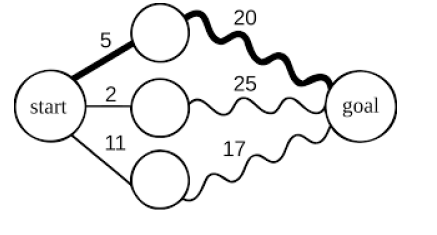
\includegraphics[width=0.5\linewidth,keepaspectratio]{dsa12}
\end{center}				
\end{frame}

%%%%%%%%%%%%%%%%%%%%%%%%%%%%%%%%%%%%%%%%%%%%%%%%%%%%%%%%%%%%%%%%%%%%%%
\begin{frame}[fragile]
	\frametitle{Knapsack}
	
	\begin{columns}[T]
		\column{0.5\linewidth}		
			\begin{itemize}
				\item We have a weights array and a values array, where we want to choose those values which will return us 
the maximum weight sum (within the limit). 
				\item $max weight == 0$ will be the base case. 				
\item At every step, we have 2 
CHOICES:
			\begin{itemize}
				\item Include the value: Take value from $values[index] +$ move ahead 
				\item Exclude the value: Just move ahead 
			\end{itemize}
			\item We’re re-calculating a lot of states. Use memoization.
			\end{itemize}
		\column{0.5\linewidth}
\begin{lstlisting}
knapsack(weights [], values [], maxWeight = 0, index = i, memo_set = set()) 
{ 
  if(i ==  weights.length || maxWeight == 0){ 
  return  0; 
  } 
 
  //include the ith item 
  int include = v[i] + knapsack(w, v, maxWeight - weights[i], i+1); 
  // don't include 
  int exclude =  knapsack(w, v, maxWeight, i+1); 
 
  return Math.max(include, exclude); 
} 
\end{lstlisting}			
		
		
	\end{columns}		
\end{frame}

%%%%%%%%%%%%%%%%%%%%%%%%%%%%%%%%%%%%%%%%%%%%%%%%%%%%%%%%%%%%%%%%%%%%%%
\begin{frame}[fragile]
	\frametitle{Knapsack}
	

			\begin{itemize}
			\item We’re re-calculating a lot of states. Use memoization.
			\item We set the key and max value in the set, and then use that in the base case to return when that 
condition is reached. 
			\end{itemize}
			
\begin{lstlisting}
knapsack(weights [], values [], maxWeight = 0, index = i, memo_set = set()) 
{  
  if(i ==  weights.length || maxWeight == 0){ 
    return  0; 
  } 
 
  String key = maxWeight + "unique Key" + i; 
 
  // check if the key is inside this set 
  if(memo_set.containsKey(key)){ 
    return memo_set.get(key); 
  } 
 
  //include the ith item 
  int include = v[i] + knapsack(w, v, maxWeight - weights[i], i+1, set); 
  // don't include 
  int exclude =  knapsack(w, v, maxWeight, i+1, set); 
  memo_set.put(key,Math.max(op1, op2)); 
  return Math.max(include, exclude); 	
\end{lstlisting}			
		
		
\end{frame}
